\chapter{Estado del arte y fundamentos teóricos}

Antes de empezar a escribir código, se deben entender los conceptos fundamentales que permitirán llevar a cabo este Trabajo de Fin de Grado.

Dagger busca mejorar el desarrollo de un ciclo completo de CI/CD de una aplicación. Por lo tanto, es fundamental definir los conceptos de \textit{Continuous Integration} y el \textit{Continuous Delivery}. Una vez se comprenda a qué se refieren esos términos, se podrán entender los métodos y tecnologías convencionales que permiten implementar dichos procesos. Será entonces cuando se pueda introducir Dagger, un herramienta innovadora para implementar \textit{pipelines}.

\section{CI/CD}

CI/CD son las siglas de \textit{Continuous Integration}/\textit{Continuous Delivery} o, en casos más específicos, este último también se puede conocer como \textit{Continuous Deployment}. Se trata de un conjunto de pasos automatizados, utilizados en el desarrollo de \textit{software} para llevar el código desde su implementación inicial hasta el despliegue de la aplicación. Estos pasos incluyen:

\begin{itemize}
  \item Integración de cambios en el código.
  \item Compilación de la aplicación con los cambios realizados.
  \item Realización de pruebas.
  \item Creación y publicación de imágenes de Docker y paquetes NPM.
  \item Despliegue de la aplicación.
\end{itemize}

\subsection*{\textit{Continuous Integration}}
\label{subsec:CI}

Se basa en la integración de código de manera constante, día a día, en un repositorio compartido por programadores. Cada uno de los programadores realiza cambios en el código y lo integra en el repositorio. Una vez se realizan cambios, estos deben pasar una serie de pruebas antes de poder ser incorporados de forma definitiva en el código fuente de la aplicación (Figura \ref{fig:ci}).

\begin{figure}
  \centerline{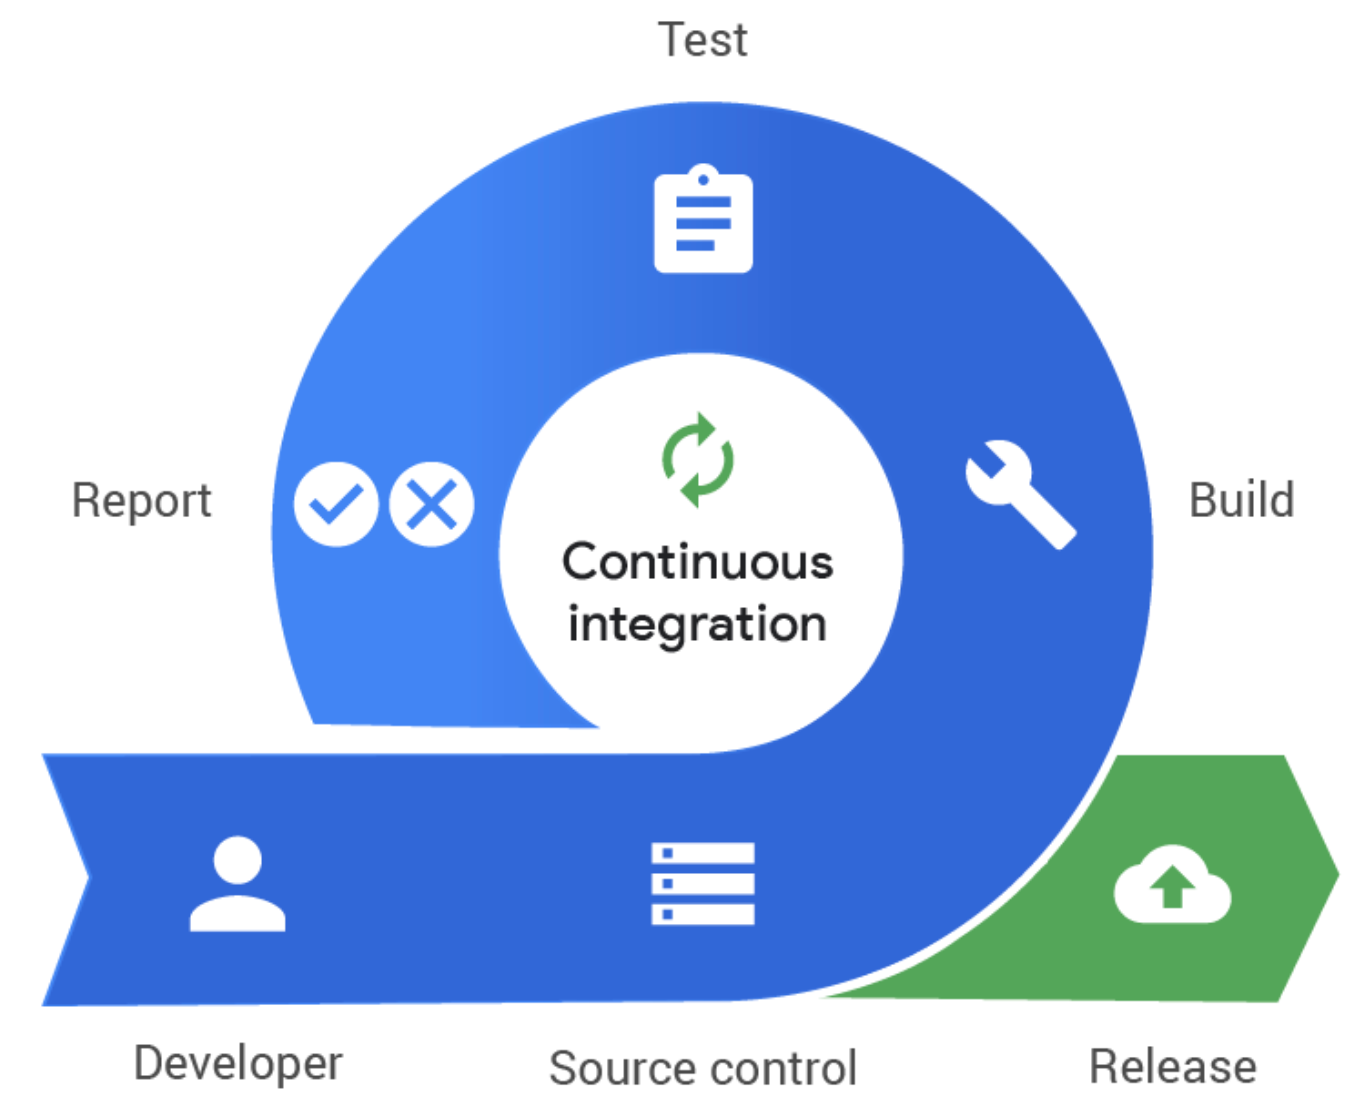
\includegraphics[width=10cm]{figuras/ci}}
  \caption{Proceso de integración continua\cite{img:ci}.}
  \label{fig:ci}
\end{figure}

Desde hace años se utilizan sistemas de control de versiones para gestionar el código de cualquier proyecto. Este tipo de herramientas permite a un equipo controlar el estado del código en cada momento, siendo capaces de conocer el historial de los cambios realizados, saber quién ha hecho cada cambio y tener la capacidad de revertir alguna modificación en el caso de ser necesario. La herramienta de control de versiones más utilizada hoy en día, y la que se utiliza en este proyecto, es Git\cite{git}.

La integración de código en un repositorio no se trata simplemente de modificar una porción de un archivo y subirlo. El código debe ser probado antes de intregrarlo completamente en el núcleo de la aplicación. Durante el proceso de integración continua, cada vez que se modifica algo de código, se debe:

\begin{itemize}
  \item Construir la aplicación.
  \item Pasar pruebas de funcionalidad.
  \item Pasar el \textit{linting} del propio código, es decir, verificar que el código cumpla ciertos estándares de estilo.
  \item Reportar cualquier error en el caso de que exista.
\end{itemize}

Todo lo anterior se debe realizar de manera automatizada, con el fin de integrar el código modificado en el repositorio lo más rápido posible, evitando en la medida de lo posible la intervención humana.

\subsection*{\textit{Continuous Delivery}}
\label{subsec:CD}

Tras haber construido la aplicación durante el proceso de integración continua, toca desplegar la aplicación. El despliegue automático de nuevas versiones de una aplicación que han pasado el ciclo de CI se conoce como ``despliegue continuo'' (Figura \ref{fig:cd}).

Esto tiene como requisito que la aplicación que se está construyendo tenga el despliegue como uno de los pasos en su ciclo de vida, lo cual no tiene por qué ser así. En este Trabajo de Fin de Grado sí que ocurre, ya que la aplicación de prueba que se construye es una página web, junto con una API y una base de datos.

Es necesario que exista relación entre los desarrolladores y los encargados de desplegar la aplicación. Sin embargo, hoy en día encontramos en muchas empresas un conjunto de metodologías conocidas como DevOps\cite{devops}, lo cual implica que ciertos integrantes de un equipo deben tener conocimiento tanto del desarrollo de la aplicación como del despliegue de la misma.

Esta transición a la cultura DevOps permite a los equipos desplegar sus aplicaciones más fácilmente. Además, incluye la necesidad de que el despliegue sea una parte muy importante en el proceso de desarrollo.

Al igual que en la integración continua, en este ciclo también es necesario automatizar el proceso despliegue de una aplicación. Esto permitirá disminuir la posibilidad de error humano.

Con el despliegue continuo podemos tener \textit{feedback} más rápido por parte del usuario, lo que permitirá mejorar y corregir errores más rápidamente. Además, se despliegan con más frecuencia cambios realizados en la aplicación, por lo que los errores en producción son menos probables y, en el caso de que los haya, más fáciles de corregir. Esto también es gracias a llevar un historial de los cambios mediante una herramienta de control de versiones como Git.

\begin{figure}
  \centerline{
\includegraphics[width=17cm]{figuras/cd}}
  \caption{Proceso de despliegue continuo\cite{img:cd}.}
  \label{fig:cd}
\end{figure}

\subsection*{GitOps \& ArgoCD}

Basándose en la filosofía DevOps, mencionada antes, que abarca tanto el ciclo de CI como el de CD, existen un conjunto de prácticas en las que se utiliza Git como fuente de verdad para la gestión de la infraestructura y las aplicaciones. Esto es conocido como GitOps\cite{gitops}. Utilizar Git como la única fuente de información permite gestionar de manera consistente la infraestructura de las aplicaciones. Realizar cambios en un repositorio produce la ejecución de \textit{workflows} o secuencias de acciones de CI/CD, los cuales reflejan en el entorno de despliegue correspondiente los cambios que se han llevado a cabo.

La herramienta que realiza estas prácticas de GitOps, y que se utiliza en este Trabajo de Fin de Grado, es ArgoCD\cite{argocd}. ArgoCD es una herramienta que, como su nombre indica, facilita el despliegue continuo. Supervisa repositorios de Git para aplicar los cambios que se realizan en ellos automáticamente en el \textit{cluster} (ver Sección \ref{tech:argocd}).

\section{Ecosistema de herramientas}

Un \textit{pipeline} moderno se compone de diferentes tipos de herramientas, cada una con sus características y finalidades. Se pueden agrupar en los ciclos que se han indicado anteriormente, CI y CD. El grupo de herramientas de CI facilitan la construcción y empaquetado de la aplicación que se va a construir, mientras que las de CD permiten desplegar la aplicación empaquetada previamente.

\subsection*{Herramientas de construcción y empaquetado}

Como cabe esperar, los pasos mencionados en la Sección \ref{subsec:CI}, que forman parte de la integración continua, van a depender del tipo de aplicación que se esté construyendo, y de las tecnologías que se estén utilizando. Además, esta secuencia de acciones pueden incluir unos pocos comandos en trabajos o proyectos sencillos, o necesitar varios \textit{scripts} complejos en el caso de aplicaciones más avanzadas. Por lo tanto, es necesario tener una herramienta de construcción que permita realizar los pasos mencionados anteriormente, sin la necesidad de memorizar cada uno de los comandos o \textit{scripts} que hay que ejecutar.

\subsubsection*{Make}
\label{subsec:make}

Para ello existe \texttt{make}\cite{make}, una aplicación de línea de comandos que permite definir bloques de comandos o reglas, aportando a cada bloque un nombre u objetivo que se pretende obtener ejecutando dicha regla. Se suele crear un archivo llamado \texttt{Makefile} para definir todas las reglas que se precisen.

Un ejemplo muy típico de compilación de un programa escrito en \texttt{C} sería el que se puede observar en el Listing \ref{lst:make}.

\begin{listing}[!ht]
  \begin{minted}{basemake}
# Compiler
CC = gcc

# Compiler options
CFLAGS = -Wall -g

# Final executable name
TARGET = my_program

# The object files (.o) needed by the program
# Make infers automatically that .o depends on the corresponding .c
OBJS = main.o hello.o

# --- Rules ---

# The first rule is the one executed by default with *make*
# It declares that to create the TARGET, it needs the OBJS
$(TARGET): $(OBJS)
  $(CC) $(CFLAGS) -o $(TARGET) $(OBJS)

# *.PHONY* tells Make that *clean* is not a file
.PHONY: clean
clean:
  rm -f $(TARGET) $(OBJS)
\end{minted}
\caption{Makefile para compilación de un programa en C}
\label{lst:make}
\end{listing}

\subsubsection*{Just}
\label{subsec:just}

En este Trabajo de Fin de Grado se utiliza una herramienta de construcción más moderna y polivalente llamada \texttt{just}\cite{just}. Este software tiene la misma finalidad que \texttt{make}, ejecutar comandos específicos de un proyecto. Pero este incluye muchas más funcionalidades (ver Sección \ref{tech:just}).

En la Listing \ref{lst:just} se puede ver que se hace uso de comandos y sintaxis propios de sistemas UNIX (por ejemplo, Bash), por lo que se trata de un requisito de software contar con un entorno UNIX o compatible (Linux, macOS, WSL, etc.) para su correcta ejecución.

\begin{listing}[!ht]
  \begin{minted}{basemake}
# --- ALIASES ---
# Defines shortcuts (aliases) for longer commands.
alias dv := down_vol

# --- DEFAULT RECIPE ---
# This is the recipe that runs if you just type 'just' in the
# terminal.
# By default, it invokes the 'just -l' recipe, which lists all
# available recipes.
# The '_' prefix indicates that it is a helper recipe, not
# intended to be called directly by the user.
_default:
  just -l

# --- INTERNAL (PRIVATE) RECIPES ---
_build_zoo_base:
  #!/usr/bin/env bash
  if [[ "$(docker images -f reference=zoo-base | wc -l | xargs)" != "2" ]]
  then
    docker build --target base -t zoo-base .
  fi

# Accepts two parameters: 'entrypoint' and 'command'.
_run entrypoint command:
  # '@' at the beginning of a command line prevents 'just' from
  # printing the command before executing it.
  @just _build_zoo_base
  docker run --rm -w /app -v $PWD:/app --env-file .env --entrypoint={{entrypoint}} zoo-base {{command}}

# --- PUBLIC RECIPES ---
init:
  @just _run "yarn" "install"

down_vol:
  docker compose down -v
\end{minted}
\caption{Extracto de justfile utilizado en el proyecto. También referenciado en la Sección \ref{tech:just}.}
\label{lst:just}
\end{listing}

\subsubsection*{Docker}
\label{subsec:docker}

Docker es una herramienta que permite empaquetar aplicaciones, creando imágenes con las dependencias necesarias para que la aplicación se lance sin problemas. Las imágenes generadas se pueden ejecutar, creando contenedores, que son entornos completamente aislados del contexto de la máquina en la que han levantado. Estos contenedores son muy ligeros en cuanto a espacio y uso de recursos, ya que almacenan únicamente lo necesario para correr el \textit{software} que queremos desplegar (ver Sección \ref{tech:docker}).

La mayor ventaja que proporciona el empaquetado de aplicaciones con Docker es la portabilidad. Aunque hay que tener en cuenta la arquitectura de la máquina, las imágenes se pueden lanzar en cualquier entorno con Docker instalado, lo cual evita el conocido problema de: ``En mi máquina funciona''.

\subsection*{Plataformas de despliegue}

\subsubsection*{Docker Compose}
\label{subsec:docker-compose}

Con Docker se es capaz de gestionar varios servicios desplegados en distintos contenedores. Pero existe una herramienta que apareció poco después y que facilita esta tarea, llamada ``Docker Compose''\cite{docker-compose}. Esta permite desplegar entornos con múltiples contenedores para desarrollar localmente (ver Sección \ref{tech:docker-compose}).

Docker Compose no es una plataforma de producción, se utiliza principalmente con el fin de desarrollar de manera local, y es muy útil en el caso de querer hacer pruebas rápidas de una aplicación sencilla. Se puede tomar como un precursor conceptual a la orquestación más compleja que realiza Kubernetes.

\subsection*{Kubernetes, Helm \& KinD}
\label{subsec:k8shelm}

El proyecto Kubernetes nació un año después que Docker. Es una herramienta de \textit{software} que permite orquestar contenedores. Gestiona el ciclo de vida de las aplicaciones en contenedores que viven en un \textit{cluster}. Entre sus características principales destacan:

\begin{itemize}
  \item Escalado automático.

    Aumenta o disminuye automáticamente el número de contenedores en ejecución. Esto va a depender de la cantidad de réplicas de una misma aplicación que se hayan indicado en su configuración. Kubernetes siempre va a intentar mantener el estado del \textit{cluster} cumpliendo los parámetros que se indicaron en las plantillas de configuración de cada uno de los servicios.

  \item Autorreparación.

    Si un contenedor falla, se reinicia o se reemplaza por otra instancia del mismo servicio, garantizando la continuidad de este.

  \item Descubrimiento de servicios y balanceo de carga.

    Se exponen los contenedores entre ellos y/o a Internet. Además, permite distribuir el tráfico de red, evitando así sobrecargas.
\end{itemize}

Más información en la Sección \ref{tech:k8s}.

Complementando a Kubernetes tenemos Helm (Figura \ref{fig:helm}), que se trata de un gestor de paquetes para Kubernetes. Su propósito es ayudar a instalar recursos y administrar el ciclo de vida de las aplicaciones de Kubernetes. Además, las Charts de Helm son formatos de archivos YAML que permiten definir los objetos de Kubernetes de una manera dinámica. Esto facilita la definición de aplicaciones mucho más complejas .

\begin{figure}
  \centerline{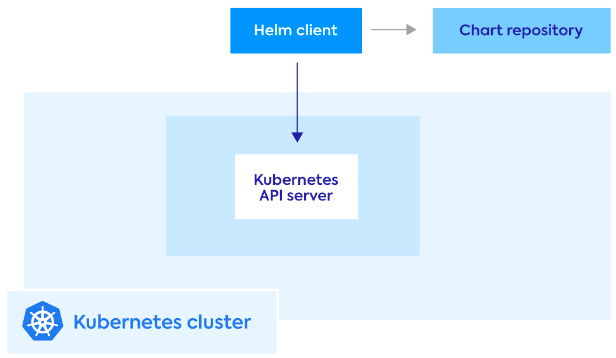
\includegraphics[width=10cm]{figuras/helm}}
  \caption{Arquitectura de Helm\cite{img:helm}.}
  \label{fig:helm}
\end{figure}

Para desplegar una aplicación de Kubernetes es necesario tener un \textit{cluster} preparado para soportar este tipo de recursos. Un \textit{cluster} de Kubernetes es un conjunto de máquinas o nodos que trabajan juntos con el fin de ejecutar y gestionar aplicaciones que corren dentro de contenedores. Para crear los \textit{clusters} en los que se despliega la aplicación se utiliza KinD\cite{kind}.

KinD (\textit{Kubernetes in Docker}) permite crear \textit{clusters} de Kubernetes de manera local. Se utiliza esta herramienta debido a su sencillo uso. Simplemente utilizando el comando que se muestra en el Listing \ref{lst:kindcc} se puede construir un \textit{cluster} en el que desplegar cualquier aplicación de Kubernetes.

\begin{listing}[!ht]
  \begin{minted}{bash}
kind create cluster
  \end{minted}
  \caption{Comando para crear un cluster con KinD}
  \label{lst:kindcc}
\end{listing}

Para gestionar los propios recursos de Kubernetes que existen dentro del \textit{cluster} se utiliza la herramienta \texttt{kubectl}\cite{kubectl}. Se trata de un CLI oficial de Kubernetes que permite comunicarse con el controlador principal del \textit{cluster}, utilizando la API de Kubernetes. Un ejemplo de uso se puede observar en el Listing \ref{lst:kubectl}.

\begin{listing}[!ht]
  \begin{minted}{bash}
kubectl apply -f "argo/argo_dev.yaml" --context kind-dev
  \end{minted}
    \caption{Aplicar la configuración de ArgoCD con kubectl}
    \label{lst:kubectl}
\end{listing}

El uso de estas dos herramientas se ve más en detalle en la Sección \ref{subsec:clusters}.

\section{Dagger}

\begin{figure}
  \centerline{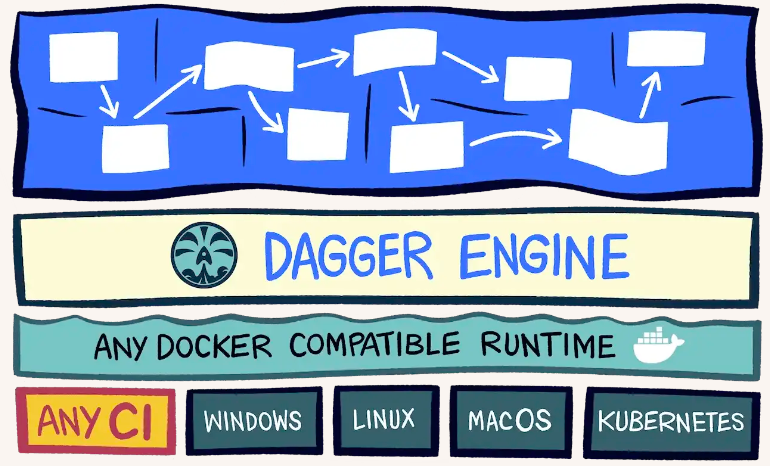
\includegraphics[width=10cm]{figuras/dagger}}
  \caption{\textit{Pipelines} con Dagger sobre un \textit{runtime} compatible con Docker\cite{img:dagger}.}
  \label{fig:dagger}
\end{figure}

Dagger es el pilar fundamental de este Trabajo de Fin de Grado. Se trata de un kit de desarrollo de \textit{software} que permite a los desarrolladores crear \textit{pipelines} CI/CD y ejecutarlos en cualquier sitio.

La principal idea de los creadores de Dagger es poder crear \textit{pipelines} portables, que no sea necesario implementarlos de nuevo cada cierto tiempo debido a cambios en el entorno de desarrollo o de pruebas. Esta portabilidad se consigue permitiendo a los desarrolladores utilizar cualquier \textit{runtime} de OCI para ejecutar las funciones que forman parte del SDK\cite{sdk} de Dagger, así como las que definen los propios desarrolladores. Además, desde el principio se ha evitado el uso de archivos YAML, que está siendo el lenguaje de configuración más utilizado por parte de la mayoría de aplicaciones.

\subsubsection*{CUE}
\label{subsec:cue}

Dagger comenzó utilizando un lenguaje de configuración muy potente llamado CUE\cite{cue}. Este se podría ver como una extensión de JSON, pero con más funcionalidades. Todo lo escrito en JSON se puede traducir a CUE, pero no al revés. En el Listing \ref{lst:cue} se puede ver un ejemplo de código de Dagger en el que se utiliza CUE para lanzar un ``plan''. En él se descarga la imagen de Docker de Alpine y se almacena en un registro levantado en la máquina local.

\begin{listing}[!ht]
  \begin{minted}{go}
package main

import (
    "dagger.io/dagger"
    "universe.dagger.io/docker"
)

dagger.#Plan & {
    actions: {
        pull: docker.#Pull & {
            source: "alpine"
        }
        push: docker.#Push & {
            image: pull.output
            dest:  "localhost:5042/alpine"
        }
    }
}
  \end{minted}
  \caption{Código de Dagger con CUE}
  \label{lst:cue}
\end{listing}

Esta es la primera vez que se pueden ejecutar \textit{pipelines} definidas de manera programática, ejecutadas sobre un \textit{runtime} de OCI, y de manera relativamente funcional. Además, se puede ejecutar toda la secuencia de acciones de manera local, permitiendo realizar pruebas y buscar errores sin necesidad de hacer uso de otras herramientas de CI como GitHub Actions\cite{github-actions}.

Además, Dagger hace un uso exhaustivo de la caché. Todas las acciones son cacheadas automáticamente. Esto es una funcionalidad muy útil, ya que va a hacer que un \textit{pipeline} se ejecute en algunos casos un 90\% más rápido, como ha ocurrido en pruebas realizadas en este Trabajo de Fin de Grado, que se comentan más adelante. Si se pone como ejemplo la ejecución de tests sobre una aplicación, la primera vez que se lanza el \textit{pipeline}, este tiene que ejecutarse completamente:

\begin{enumerate}
  \item Instalar las dependencias.
  \item Compilar la aplicación.
  \item Correr los tests.
\end{enumerate}

Dependiendo del tipo de aplicación y de la conexión a Internet, esto puede tardar desde unos segundos hasta varios minutos. Pero con Dagger solo ocurre una vez. La primera vez. Gracias a la caché, todas las acciones repetitivas, como la instalación de dependencias o la compilación de la aplicación, se almacenan en la caché, ahorrando así mucho tiempo a la hora de realizar pruebas de cualquier tipo. Mientras tanto, con otras herramientas se tendría que esperar siempre la misma cantidad de tiempo para cada una de las veces que se quiere lanzar el \textit{pipeline}. Además, Dagger puede ejecutar estas acciones de manera local, mientras que utilizando métodos convencionales habría que depender de aplicaciones que pueden fallar o no estar disponibles en cierto momento.

\subsubsection*{CI/CD como código}
\label{subsec:cicd-code}

Dagger ha querido ir más allá pensando que los desarrolladores deberían ser capaces de crear sus \textit{pipelines} de la misma manera que crean sus aplicaciones: escribiendo código. Es así como nace el SDK de Go\cite{go} para Dagger, el cual se utiliza en este Trabajo de Fin de Grado. Go es un lenguaje de programación con muchos casos de uso. Desde la creación de servicios de red y en la nube, hasta aplicaciones CLI y desarrollo web. Es conocido también por su simplicidad en cuanto a sintaxis y por tener una librería estándar muy completa, aportando muchas de las herramientas necesarias para realizar proyectos comunes. Además, facilita la implementación de programación concurrente, gracias a las \textit{goroutines}, similares a los hilos de ejecución de un sistema operativo, pero mucho más ligeros. En el Listing \ref{lst:daggergo} se puede observar un ejemplo de código utilizando el SDK de Go.

\begin{longlisting}
  \begin{minted}{go}
package main

import (
	"context"
	"dagger/dagger/internal/dagger"
	"fmt"
	"strconv"
)

type Backend struct {
	Name string
	Base *dagger.Container
	Secrets SecMap
}

func (m *Backend) Build(ctx context.Context) *dagger.Container {
	build := m.Base.
		WithWorkdir("/app").
		WithExec([]string{"lerna", "run", "--scope", "@vieites-tfg/zoo-backend", "build"}).
		WithExec([]string{"ncc", "build", "./packages/backend/dist/index.js", "-o", "./dist"})

	return build
}

func (m *Backend) Ctr(ctx context.Context) *dagger.Container {
	build := m.Build(ctx)

	compiled := build.File("/app/dist/index.js")
	pkgJson := build.File("/app/packages/backend/package.json")

	dag := dagger.Connect()
	back := dag.
		Container().From("node:20-alpine").
		WithExposedPort(3000).
		WithEnvVariable("NODE_ENV", "production").
		WithEnvVariable("YARN_CACHE_FOLDER", "/.yarn/cache").
		WithMountedCache("/.yarn/cache", dag.CacheVolume("yarn-cache")).
		WithWorkdir("/app").
		WithFile("/app/package.json", pkgJson).
		WithFile("/app/index.js", compiled).
		WithExec([]string{"yarn", "install", "--production"}).
		WithEntrypoint([]string{"node", "index.js"})

	return back
}
\end{minted}
  \caption{Ejemplo del SDK de Go de Dagger.}
  \label{lst:daggergo}
\end{longlisting}

Todo lo anterior hace de Go una elección excelente para empezar la lista de lenguajes de programación sobre los que el equipo de Dagger implementaría su propio SDK, que hasta el día de hoy incluyen: Typescript, Java, PHP, Node y Python. 

\subsubsection*{GraphQL}

El equipo de Dagger es capaz de desarrollar SDKs específicos para cada lenguaje tan rápidamente gracias al uso de GraphQL\cite{graphql}, un lenguaje para manipulación y consulta de datos.

\begin{figure}
  \centerline{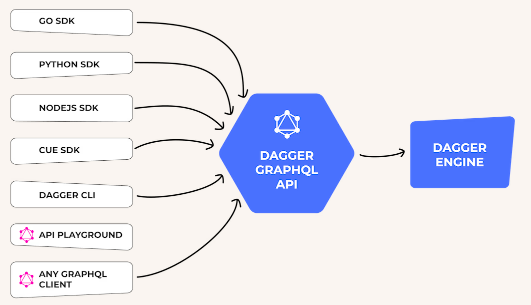
\includegraphics[width=14cm]{figuras/graphql}}
  \caption{Uso de la API de GraphQL para Dagger\cite{img:graphql}.}
  \label{fig:graphql}
\end{figure}

Se puede ver su funcionamiento en la Figura \ref{fig:graphql}. El SDK de cada uno de los lenguajes funcionan como traductores del código que escribes en dicho lenguaje a sentencias que entiende el motor de Dagger. Esto es a través de la API de GraphQL de Dagger. El motor de Dagger es el que se encarga de ejecutar las instrucciones en un entorno controlado. De esta manera, no son los propios SDKs los que corren los programas dependiendo del lenguaje, sino que funcionan como clientes de la API para traducir la secuencia de acciones y ejecutarse en un mismo entorno.

\subsubsection*{Dagger \textit{functions}}

Tras varias mejoras y nuevas versiones, el equipo de Dagger implementa las ``funciones de Dagger''. Estas funciones son el componente principal de Dagger hoy en día. Cada una de las operaciones principales de Dagger se pueden llamar a través de una función, utilizando una API. Además, estas se pueden encadenar, generando \textit{pipelines} dinámicas en una sola llamada. De esta manera, se puede decir  que gracias a Dagger se pueden programar ciclos CI/CD en uno de los lenguajes disponibles, bien conocidos en el sector.

\subsubsection*{Daggerverse}

La existencia de las funciones de Dagger permite la creación de módulos, un conjunto de funciones que toman una entrada y producen una salida en concreto. Los módulos creados por la comunidad se pueden encontrar en el Daggerverse\cite{daggerverse}. Este es el lugar en el que se comparten módulos de Dagger, los cuales se pueden reutilizar para añadir funcionalidades a otro módulo, sin necesidad de volver a crear una lógica de programación ya implementada por otra persona o equipo de desarrolladores.

\subsubsection*{CLI}

Otra funcionalidad que tiene Dagger es su CLI\cite{cli} (\textit{Command-Line Interface}). A través de ella puedes llamar a funciones de módulos de Dagger, tanto de de tu sistema de archivos local como directamente de un repositorio de Git en el que se encuentre el código fuente de un módulo.

En el Listing \ref{lst:callbackend} se muestra un ejemplo de ejecución de una de las funciones definidas en un módulo correspondiente a este Trabajo de Fin de Grado. Toda la documentación al respecto se puede encontrar en el Apéndice \ref{chap:usuario}.

\begin{listing}[!ht]
  \begin{minted}{bash}
dagger call --sec-env=file//../../.env backend service up --ports 3000:3000
  \end{minted}
  \caption{Comando para lanzar el backend del proyecto}
  \label{lst:callbackend}
\end{listing}

\subsubsection*{Resumen}

Dagger es una herramienta revolucionaria que redefine la manera de crear \textit{pipelines} de CI/CD, proporcionando la capacidad de implementar estos \textit{pipelines} programáticamente y evitar que los desarrolladores tengan que lidiar con archivos de configuración estáticos como YAML, o con la creación de diferentes \textit{scripts}. Ofrece SDKs en una variedad de lenguajes de programación, tales como Go, Python o Node, que actúan como clientes del motor central de Dagger.

Una de sus ventajas más significativas es su portabilidad, la cual se consigue al ejecutar todas las operaciones sobre un \textit{runtime} de OCI, como Docker. De esta manera se garantiza que cualquier \textit{pipeline} definido con Dagger funcione de igual manera sin importar la máquina en la que se ejecuta.

Otro de sus pilares es la gestión que hace de la caché. Dagger cachea cada una de las acciones ejecutadas. Gracias a esto, tras la primera ejecución de un \textit{pipeline}, las siguientes ejecuciones son significativamente más rápidas. Así se reducen los tiempos de espera, permitiendo a los desarrolladores trabajar más rápido.

Finalmente, la evolución hacia las ``Dagger \textit{functions}'' y la creación de módulos permite un gran nivel de reutilización. Estos módulos, que pueden ser compartidos a través del Daggerverse, junto con su CLI para invocarlos, proponen una manera muy poderosa de crear \textit{pipelines} para construir, probar y desplegar aplicaciones.
